\chapter{Introduction}\label{chp:Introduction}

	Modern software applications are often complex and have to fulfill a large set of functional and non-functional requirements. The internal behavior of such large systems cannot easily be determined on the basis of the source code. Furthermore, existing applications often lack sufficient documentation which makes it cumbersome to extend and change them for future needs. A solution to these problems can be dynamic analysis based on application-level monitoring, which allows to log the behavior of the application and to discover, for example, application-internal control flows, calling dependencies, and method response times.

	Dynamic analysis can help in detecting performance problems and faulty behavior, capacity planning, and many other areas. The Java-based \Kieker{} framework comes with tools and libraries for performance monitoring and dynamic software analysis \cite{KiekerICPE2012}. It has been designed for continuous monitoring in production systems inducing only a very low overhead. Monitoring adapters for other platforms, such as Visual Basic~6~(VB6), .NET, COBOL, and Perl are available upon request \footnote{\href{http://kieker-monitoring.net/support/}{Contact us} directly if you are interested in \Kieker{} support for these or other platforms}.  \\
	
	\noindent
	In 2011, Kieker was reviewed and accepted for distribution as part of the SPEC Research Group's repository of peer-reviewed tools for quantitative system evaluation and analysis. See \url{http://research.spec.org/projects/tools.html} for details.\\

	\NOTIFYBOX{In case that you are only interested in a quickstart example, you may want to skip directly to Chapter~\ref{chp:Quickstart-Example}.}
	
	\section{Kieker's Core Components}		
		Figure~\ref{fig:KiekerComponentDiagram} shows the framework's composition based on the two main components \KiekerMonitoringPart{} and \KiekerAnalysisPart{}. The \KiekerMonitoringPart{} component is responsible for program instrumentation, data collection, and logging. Its core is the \class{MonitoringController}. This part is explained in more detail in Chapter~\ref{chp:Kieker-Monitoring}. The component \KiekerAnalysisPart{} is responsible for reading, analyzing, and visualizing the monitoring data. Its core is the \class{AnalysisController} which manages the life-cycle of the pipe-and-filter architecture of analysis plugins, including monitoring readers and  analysis filters. This part is explained in more detail in Chapter~\ref{chp:Kieker-Analysis}.
		
		% This is the component diagram of Kieker (the satellite).
		\begin{figure}[H]\centering
			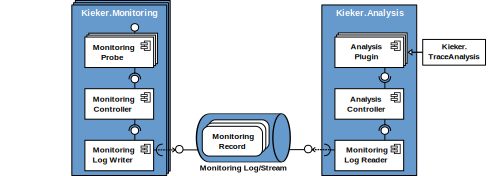
\includegraphics[width=0.81\textwidth]{images/kiekerComponentDiagram-woCloud-bw-w-record-newNames-withTraceAnalysis-colors}
			
			\caption{Overview of the framework components}
			\label{fig:KiekerComponentDiagram}
		\end{figure}
	
	\section{Download and Installation}
		
		The \Kieker{} download site\footnote{\KiekerDownloadURL{}} provides archives of the binary and source distribution, the Javadoc~API, as well as additional examples. The Java sources presented in this user guide, as well as pre-compiled binaries, are included in the \file{\exampleDir/} directory. The file \file{\mainJar{}} contains the \KiekerMonitoringPart{} and \KiekerAnalysisPart{} components, as well as the \KiekerTraceAnalysis{} tool. In addition to the \file{\mainJar{}} file, the \file{dist/} directory includes variants of this \file{.jar} files with integrated third-party libraries. Additional information on these \file{.jar} files and when to use them will follow later in this document.
		
	\section{Licensing}
		\Kieker{} is licensed under the Apache License, Version 2.0. You may obtain a copy of the license at \url{http://www.apache.org/licenses/LICENSE-2.0}. The \Kieker{} source and binary release archives include a number of third-party libraries. The \dir{lib/} directory of the release archives contains a \file{.LICENSE} file for each third-party library, pointing to the respective license text.	
		
	\section{Citing Kieker}\label{sec:ch1:citingKieker}
		When referencing Kieker resources in your publications, we would be happy if you respected the following guide lines:

		\begin{itemize}
			\item 
			When referencing the Kieker project, please cite our ICPE~2012~\cite{KiekerICPE2012} paper and/or our 2009 technical report~\cite{vanHoornRohrHasselbringWallerEhlersFreyKieselhorst2009TRContinuousMonitoringOfSoftwareServicesDesignAndApplicationOfTheKiekerFramework}. Also, you might want to add a reference to our web site (\url{http://kieker-monitoring.net/}) like~\cite{KiekerWebSite}. 
			\item 
			When referencing this user guide, e.g., when reprinting contents, please use a citation like~\cite{Kieker1.7UserGuide}.
		\end{itemize}

		\noindent At \url{http://kieker-monitoring.net/research/publications/} we provide entries for $\mathrm{B\scriptstyle IB}\!$\TeX{} and other bibliography systems.
		
	\section{Outline of this User Guide}
		The rest of this user guide is structured as followed. Chapter~\ref{chp:Quickstart-Example} contains a short quickstart example. In Chapter~\ref{chp:Kieker-Monitoring} we provide a detailed description of \KiekerMonitoringPart{} and its components, before presenting in Chapter~\ref{chp:Kieker-Analysis} the \KiekerAnalysisPart{} and its important parts. Various tools, which \Kieker{} already provides, can be found in Chapter~\ref{chp:Kieker-Tools}. The \hyperlink{hypertarget:appendix}{Appendix} finally includes additional resources, e.g., how to use the JMS writers and readers.